
\section{A szimuláció eredményei}

Kezdetben a szimuláció pontosságának megvizsgálása érdekében a már rendelkezésünkre álló bemeneti paraméterekre (melyeket Archetti is használt\cite{archetti2013evolutionary}) elvégeztünk 100-100 szimulációt, minden egyes diffúziós távolságra 1-től 5-ig.

\begin{multicols}{2}
	A bemeneti paraméterek a következőek voltak:
	\begin{itemize}[noitemsep]
		\item populáció mérete: 1000
		\item defektálók: 5\%
		\item generációk száma: 15
		\item kooperálók költsége: 0.01
		\item osztódás: nincs
	\end{itemize}
	A konstans függvények paraméterei, melyeket az elkövetkezendő szimulációk során használtunk:
	\begin{itemize}[noitemsep]
		\item $s = 2$
		\item $h = 1$
		\item $d = \frac{1}{2}D$
		\item $z = 20$
	\end{itemize}	
\end{multicols}

Megállapítottuk, hogy ugyanarra az eredményre (Ábra \ref{fig:DistChange}) jutottunk mi is mint Archetti\cite{archetti2013evolutionary}, igaz kisebb eltérések ugyan mutatkoztak. Míg mi minden esetben 100 szimulálást végeztünk, addig ő csak 10-et, így a kis eltéréseket ennek tulajdoníthatjuk.

\begin{minipage}{\linewidth}
	\centering
	\begin{multicols}{2}
		\begin{Figure}
			\centering
			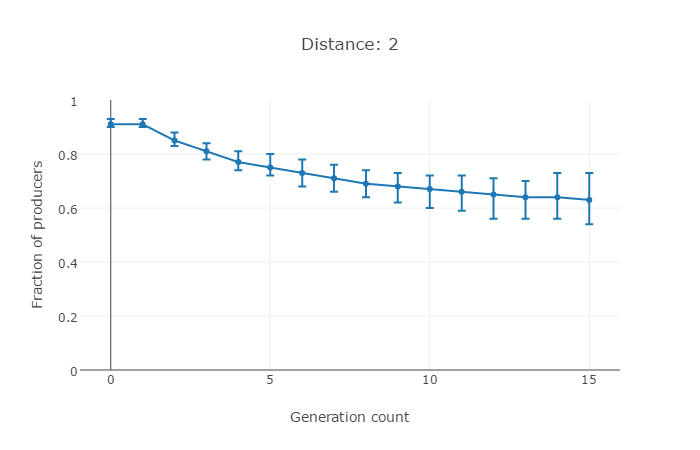
\includegraphics[width=\linewidth]{images/dist2}
		\end{Figure}
		\begin{Figure}
			\centering
			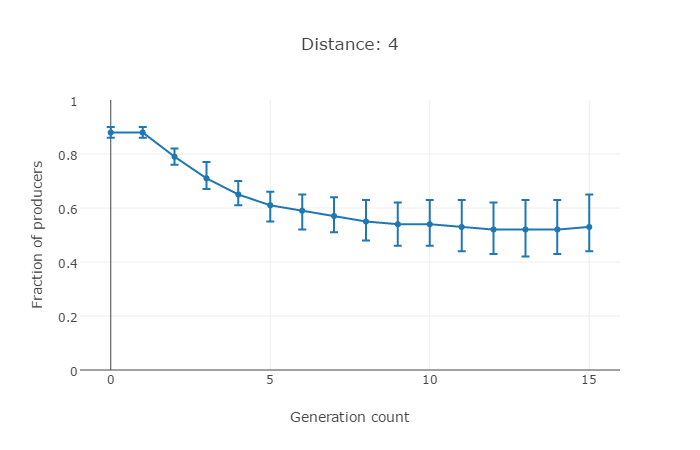
\includegraphics[width=\linewidth]{images/dist4}
		\end{Figure}
		\begin{Figure}
			\centering
			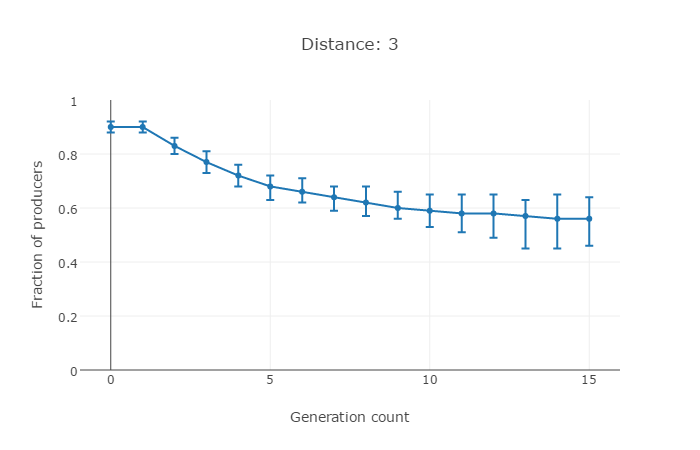
\includegraphics[width=\linewidth]{images/dist3}
		\end{Figure}
		\begin{Figure}
			\centering
			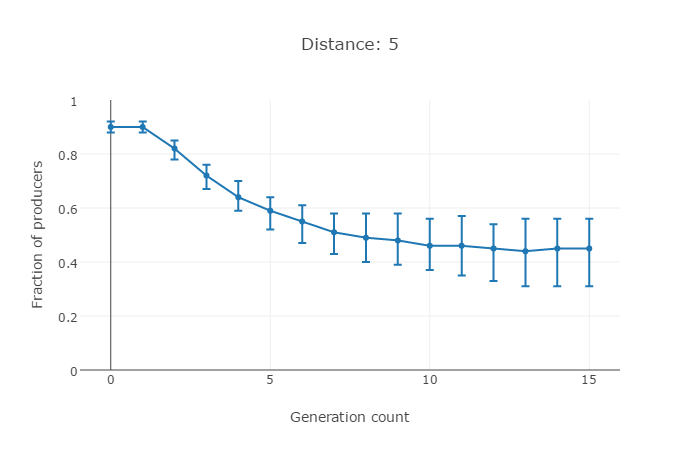
\includegraphics[width=\linewidth]{images/dist5}
		\end{Figure}
	\end{multicols}
	\captionof{figure}{Szimulációs eredmények a fenti paraméterekre\label{fig:DistChange}}
\end{minipage}\\

Ezzel projektünk első mérföldkövét leraktuk, így most már kísérletezhetünk különböző paraméterekkel, hogy megvizsgáljuk a populáció viselkedését. Egy pár esetet a következő fejezetekben tárgyalunk.

\subsection{A költség és nyereség hatása}

Mint ahogyan azt már láttuk, a kooperáló sejtek termelési költsége nagyban befolyásolja a játék végkimenetelét (Ábra \ref{fig:CoopCostChange}), ami nem nagy meglepetés, hisz minél többe kerül a termelés annál jobban megéri élősködni. Az esetek többségében a defektálás a legkifizetődőbb, de alacsony költségek mellett fenntartható egy bizonyos egyensúly is a két fél között, sőt, extrém körülmények (paraméterek) mellett az is elérhető, hogy a teljes populáció a kooperálás mellett döntsön.

\begin{minipage}{\linewidth}
	\centering
	\begin{multicols}{3}
		\begin{Figure}
			\centering
			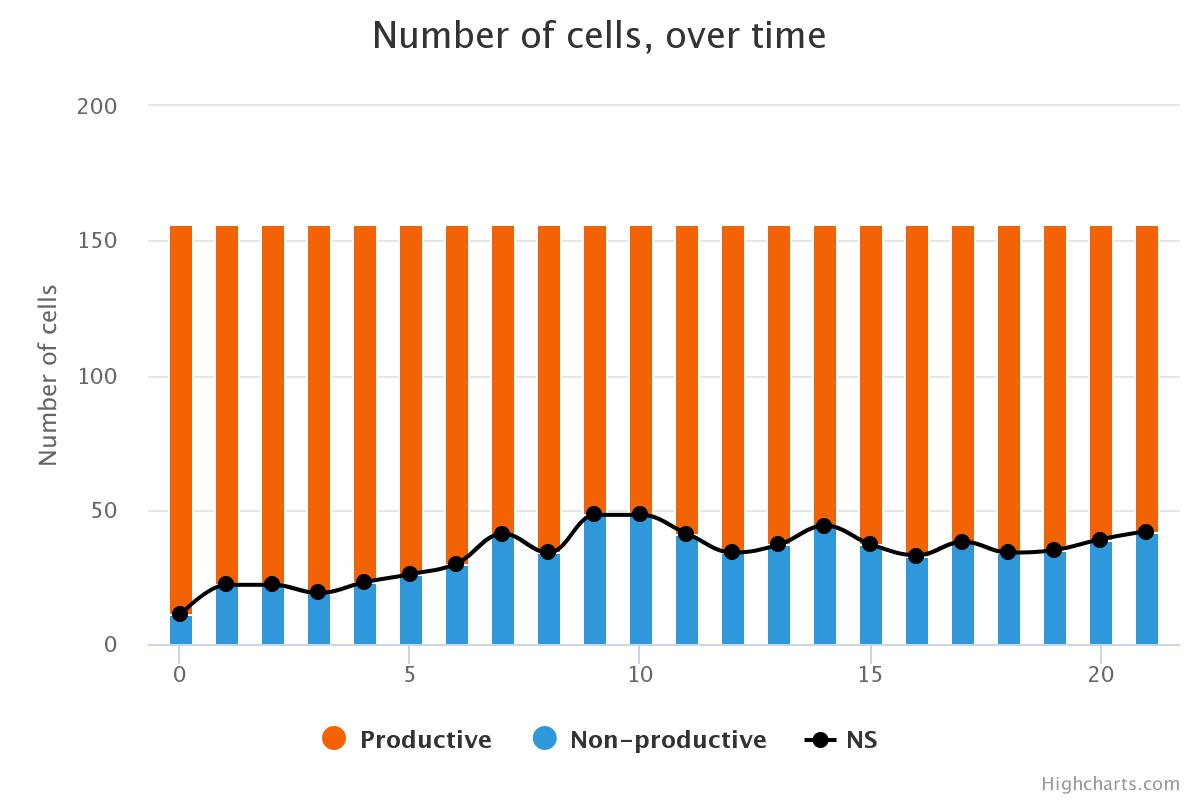
\includegraphics[width=\linewidth]{images/chart001.jpeg}
		\end{Figure}
		\begin{Figure}
			\centering
			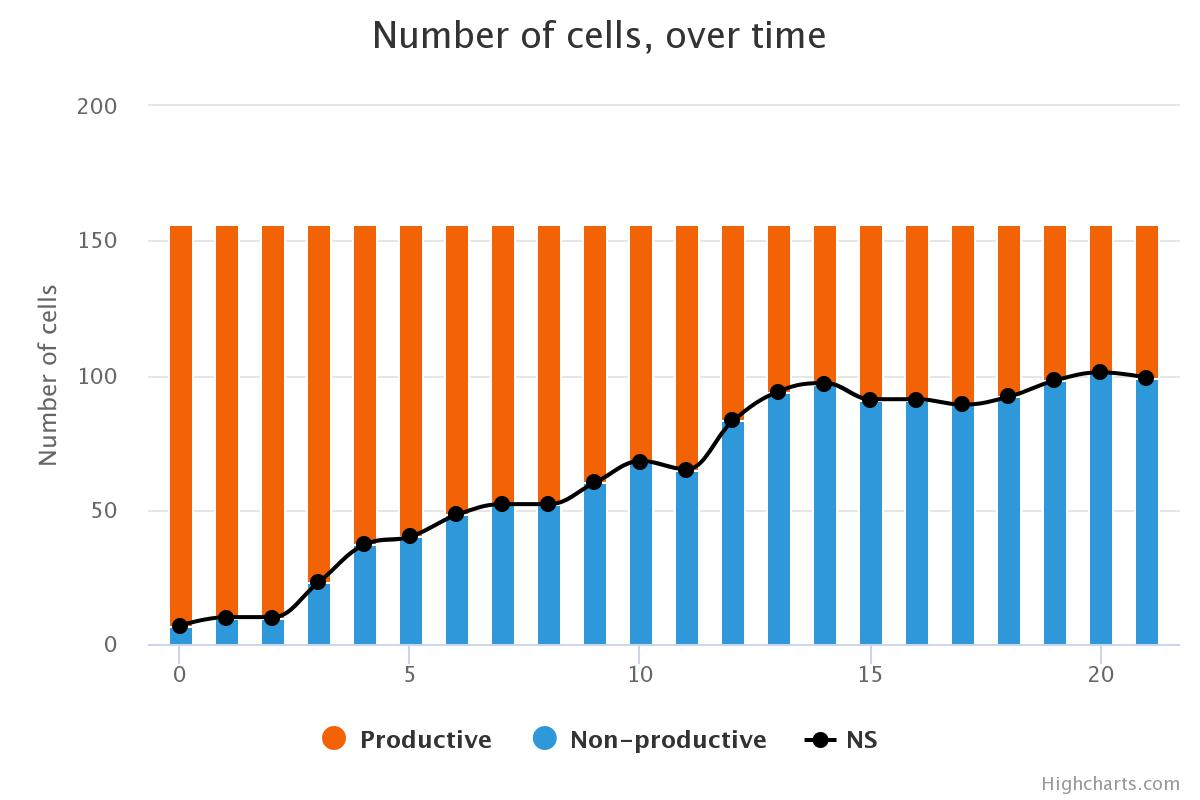
\includegraphics[width=\linewidth]{images/chart01.jpeg}
		\end{Figure}
		\begin{Figure}
			\centering
			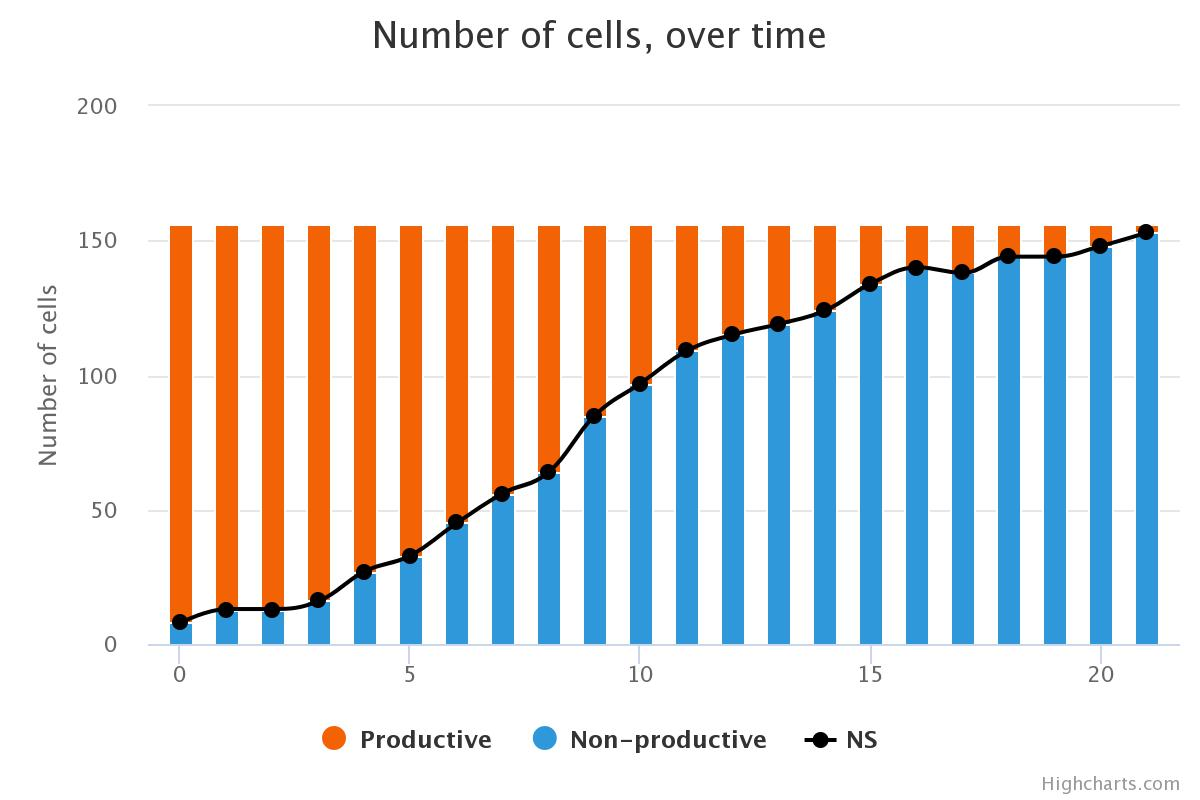
\includegraphics[width=\linewidth]{images/chart08.jpeg}
		\end{Figure}
	\end{multicols}
	\captionof{figure}{A játék végkimenetele mikor a költségek rendre 0.01, 0.1 és 0.8\label{fig:CoopCostChange}}
\end{minipage}


\subsection{Diffúziós távolság hatása}

Egyik legkényesebb paraméterünk amelyet változtatni lehet, az a diffúziós távolság, amely növelésével valósághűbb adatokat kaphatunk. Sajnos nem állnak rendelkezésünkre erre vonatkozó adatok a biológiából, így csak egy pár, már más által is használt értékekre végeztünk kísérleteket (Ábra \ref{fig:DiffDist}).

\begin{minipage}{\linewidth}
	\centering
	\begin{multicols}{2}
		\begin{Figure}
			\centering
			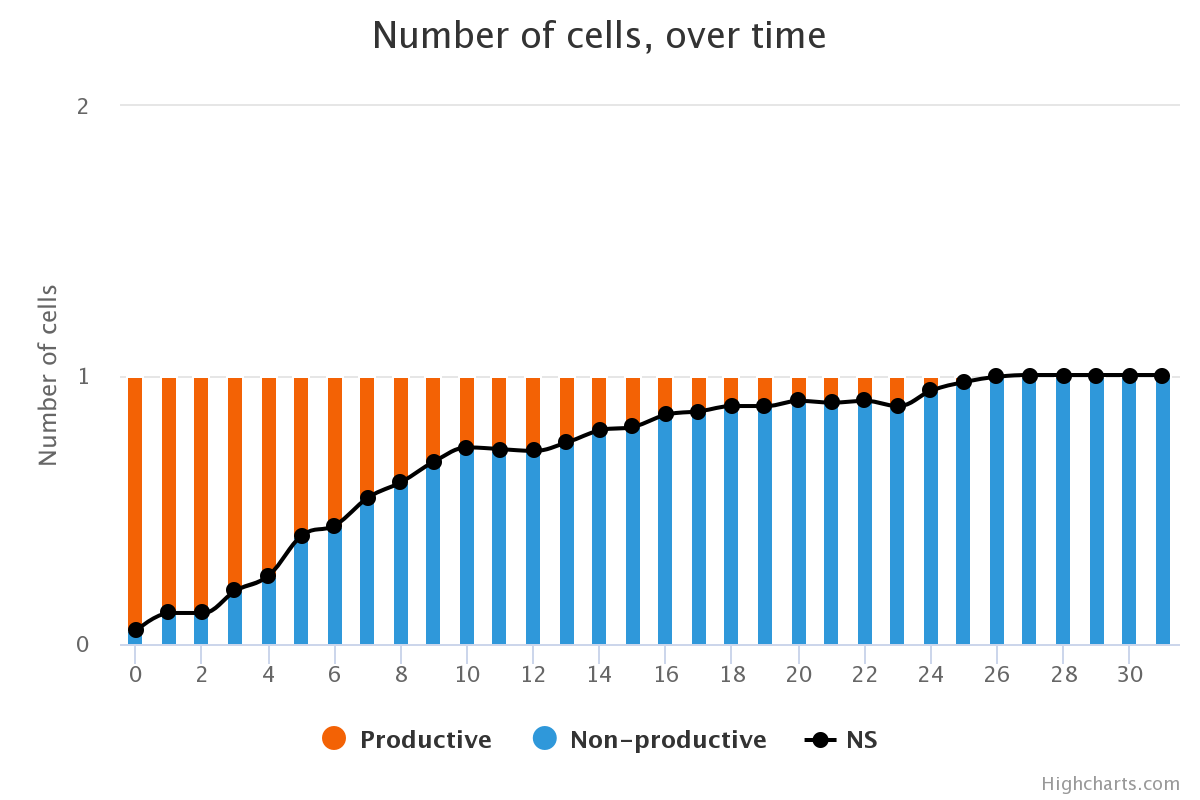
\includegraphics[width=\linewidth]{images/diffdist2}
		\end{Figure}
		\begin{Figure}
			\centering
			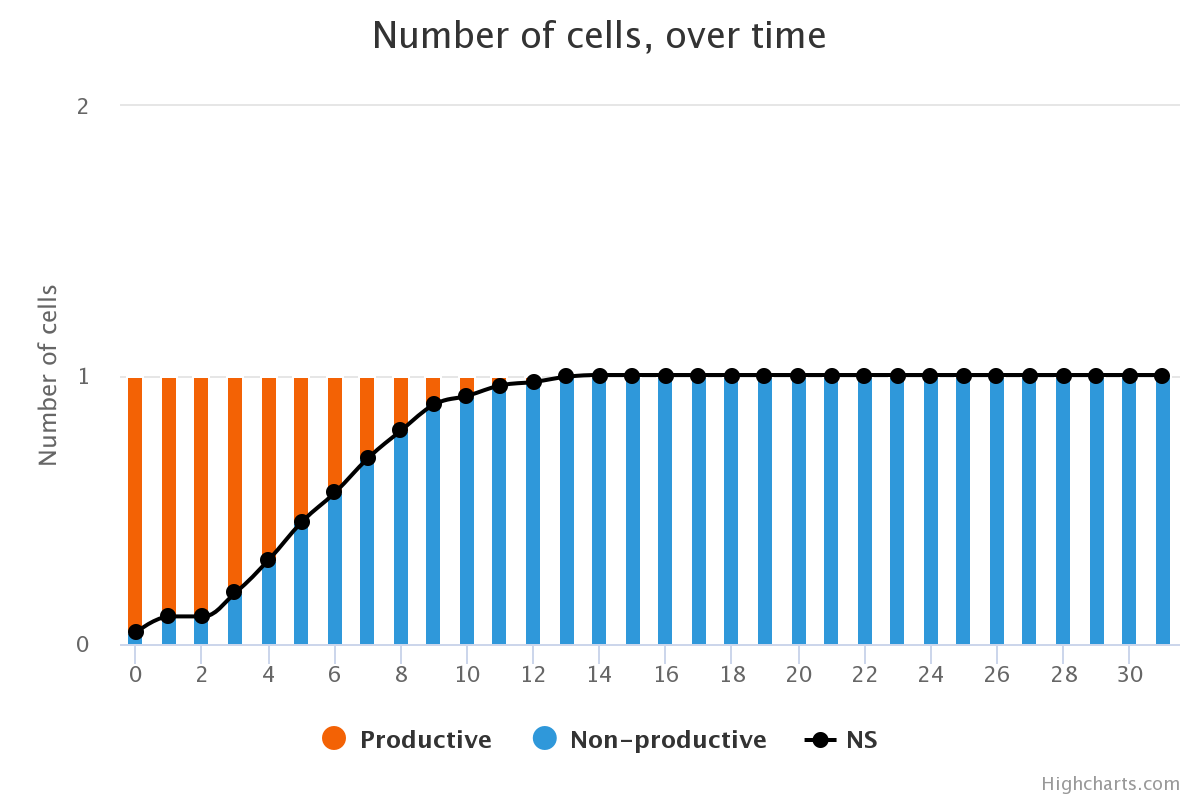
\includegraphics[width=\linewidth]{images/diffdist5}
		\end{Figure}
	\end{multicols}
	\captionof{figure}{A játék végkimenetele két diffúziós távolságra. A paraméterek: 160 sejt, 5\% defektáló, 0.3 költség, távolság: 2 illetve 5\label{fig:DiffDist}}
\end{minipage}\\


Megfigyelhető, hogy a távolság növekedésével a defektáló sejtek jóval könnyebben terjednek el, nem csak a közvetlen szomszédokat befolyásolják, hanem a távolabbiakat is. Amennyiben a távolság állandónak bizonyul, célunk pedig a defektálók kiirtása, úgy jelent esetben csak a kooperálók költségének csökkentésével tudjuk megfékezni a terjedésüket. További megvalósítandó feladataink közé tartozik egy olyan funkció mely révén ellenanyagot juttathatunk a daganatba, vagy egy terápiát alkalmazhatunk.

\subsection{Osztódásra képes populációk}

Eddigi szimulációink során a populáció mérete állandó volt, és egy adott modellt követett. Nézzük meg mi történik ha a sejtek osztódni is képesek nem csak stratégiát váltani (Ábra \ref{fig:Divide}). 

\begin{minipage}{\linewidth}
	\centering
	\begin{multicols}{2}
		\begin{Figure}
			\centering
			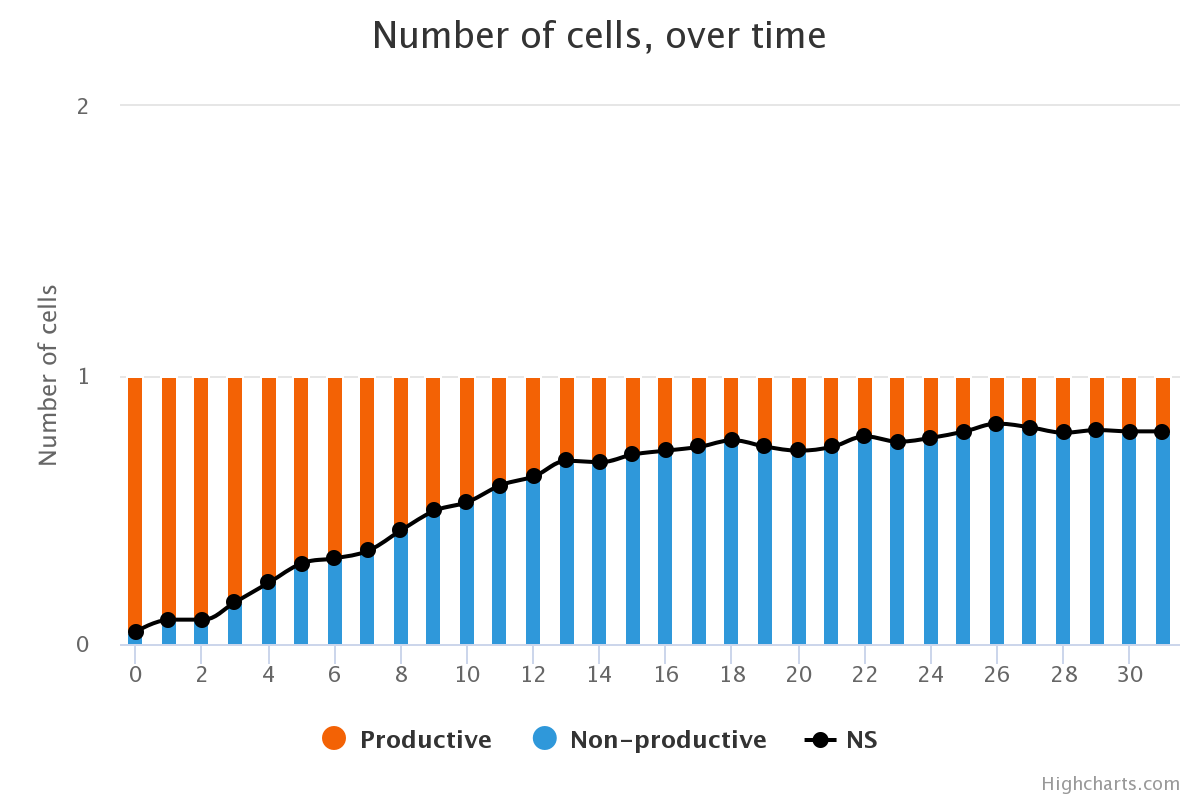
\includegraphics[width=\linewidth]{images/nemosztodik}
		\end{Figure}
		\begin{Figure}
			\centering
			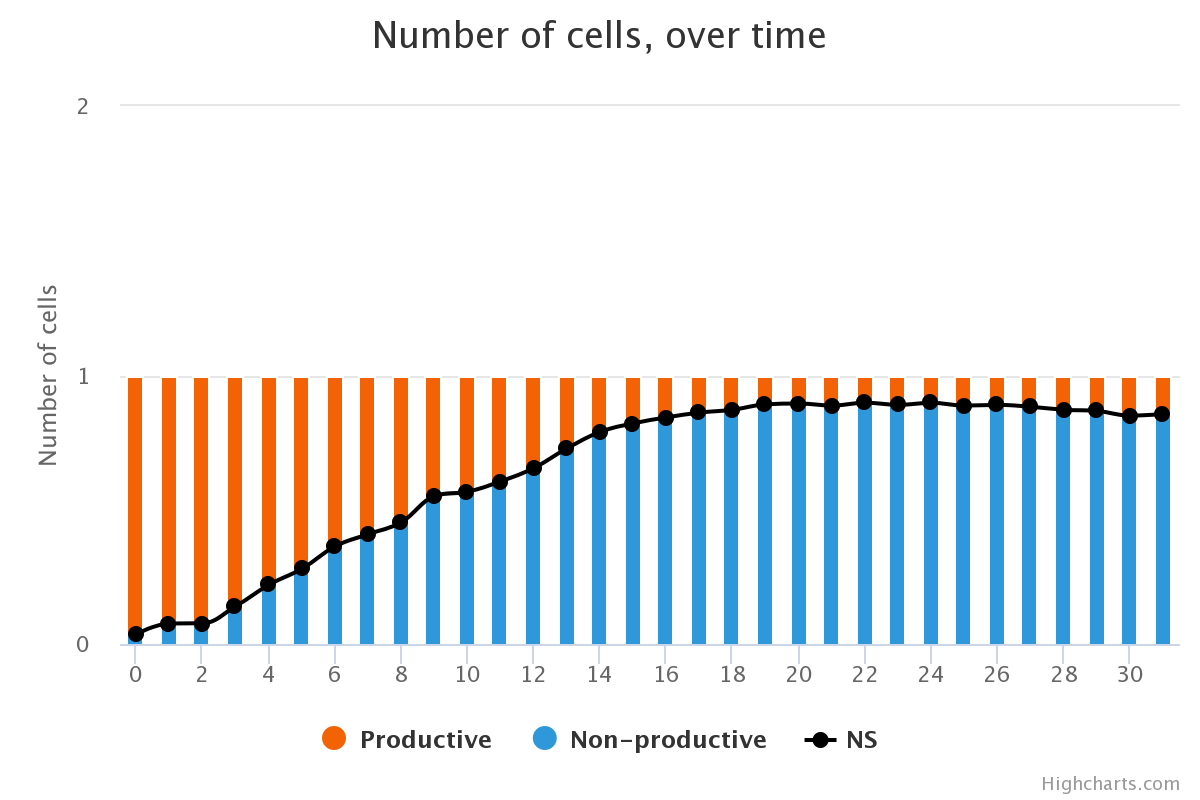
\includegraphics[width=\linewidth]{images/osztodik}
		\end{Figure}
	\end{multicols}
	\captionof{figure}{Az első esetben a sejtek nem osztódtak míg a másodikban igen \label{fig:Divide}}
\end{minipage}\\

Igaz, hogy a stratégia váltást fel lehet fogni úgy mint egy fajta osztódást, ahol az a sejt amelyik átveszi a stratégiát meghal és annak a sejtnek a másolata jön létre ugyanazon a területen akitől azt átveszi, de a valóságban a defektáló sejtek nem csak területileg terjednek el, hanem számosságban is túlnövik a kooperálókat.
Az osztódás során létrejött új sejtek képesek felgyorsítani a defektálók terjedését, de jelenleg ez a modell még nem tükrözi a valóságot teljes egészében. 

\subsection{Összegzés}

Összességében azt állíthatjuk, hogy sikerült egy olyan terméket létrehoznunk, mely megállja helyét
